
\section{서론}
\subsection{연구의 배경}

\begin{figure}[h!]
    \centering
    \begin{subfigure}[t]{0.95\textwidth}
        \centering
        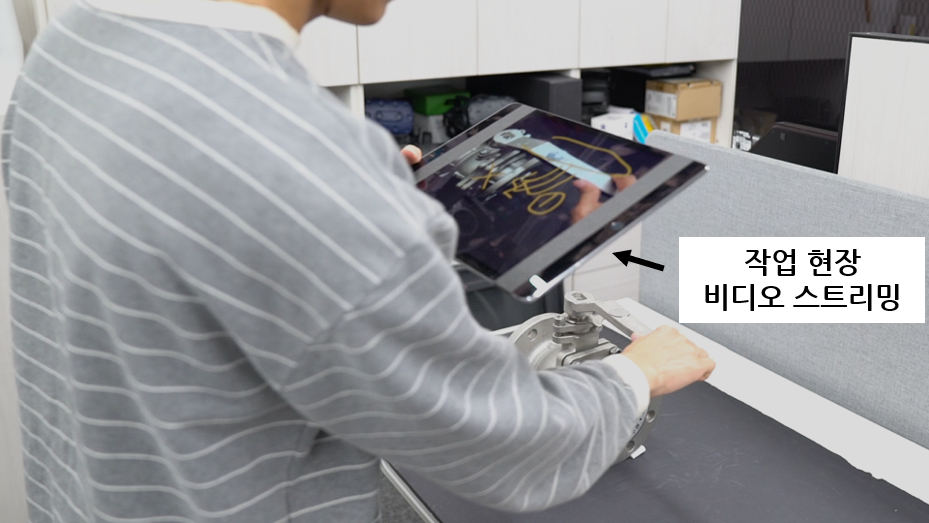
\includegraphics[width=\textwidth]{figures/remote_ar_local_site.png}
        \caption{현장 작업자의 모습: 작업 현장을 원격 작업자에게 비디오 스트리밍 하고 있음.}
        \label{fig:remote_ar_local_site}
    \end{subfigure}
    
    \par\bigskip
        
    \begin{subfigure}[t]{0.95\textwidth}
        \centering
        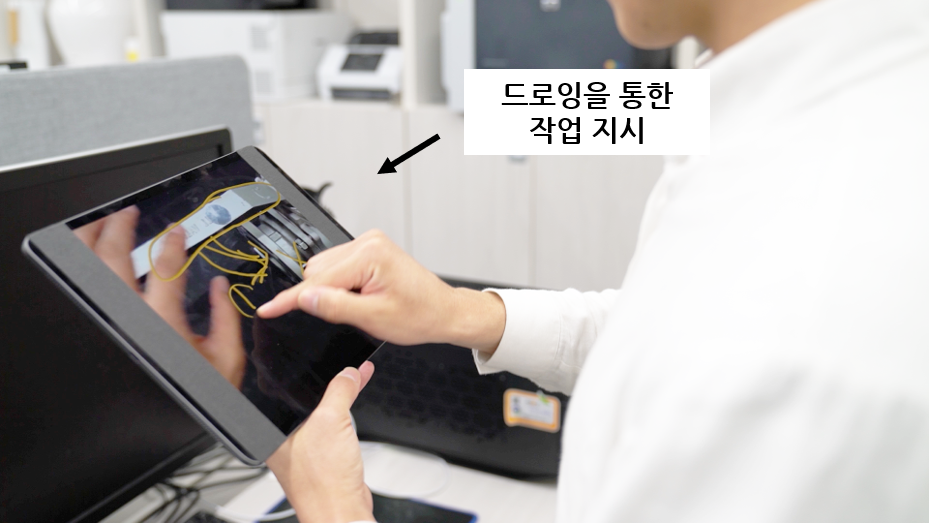
\includegraphics[width=\textwidth]{figures/remote_ar_remote_site.png}
        \caption{원격 작업자의 모습: 현장 작업자가 스트리밍하는 비디오를 통해 작업 현장의 상황을 파악하고, 그 위에 드로잉을 통해 현장 작업자가 해야될 작업을 지시하고 있음.}
        \label{fig:remote_ar_remote_site}
    \end{subfigure}
    \caption{원격 \acrshort{ar} 협업의 모습. 원격 \acrshort{ar} 협업은 원격 \acrshort{xr} 협업의 주류방식이 되었음.}
    \label{fig:remote_ar_collaobration_example}
\end{figure}


\subsection{연구의 목적}

\subsection{연구의 내용 및 구성}